\vspace*{-1cm}
\begin{figure}[!ht]
    \centering
    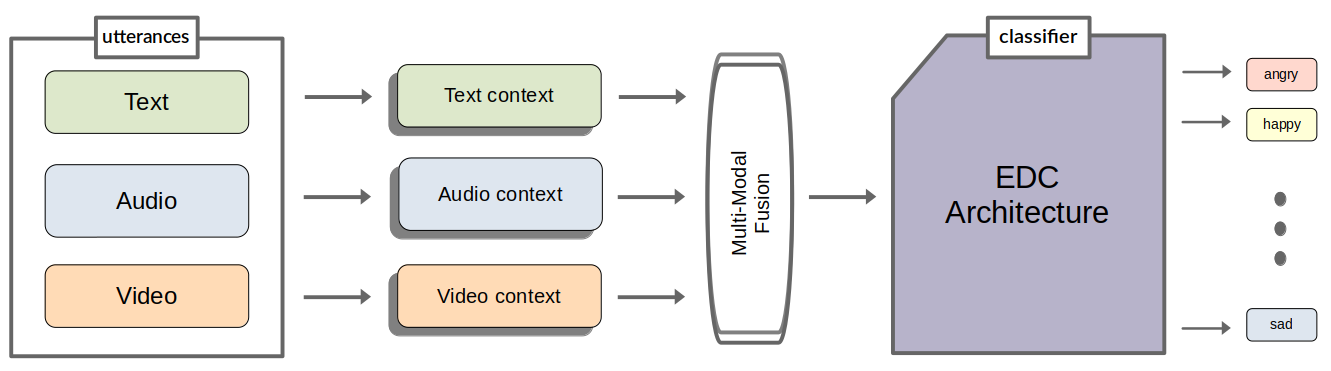
\includegraphics[width=\linewidth]{images/method_framework.png}
    \captionsetup{width=\linewidth}
    \caption{Condensed Structure of an Emotion Recognition in Conversation Framework}
    \label{fig:method_framework}
\end{figure}

\section[Techniques for Uni-Modal Feature Extraction in Emotion Recognition]{Techniques for Uni-modal Feature Extraction in \newline Emotion Recognition}
    
    \subsection{Textual Feature Extraction}
    As presented in \cite{cnn-text}, Kim offers a technique for preparing textual data for various classification tasks like sentiment analysis and determining text subjectivity. This method involves text classification by utilizing the softmax probability derived from key text features. These key features are acquired by initially concatenating vector representations of the words constituting the given text. Subsequently, a convolution operator, functioning as a filter, is applied to generate feature maps. Finally, a max pooling layer is employed to acquire the most important feature map. This innovative approach has been adopted by \cite{cmn, dialoguernn, bclstm} for textual feature representation. Specifically, in the extraction of textual modality from dyadic conversations \cite{iemocap}, \ac{cnn} with sizes 3, 4, and 5, each having 50 feature maps, are utilized. These are then subjected to max-pooling with a window of size 2 and passed through a fully connected layer with 100 neurons to represent the textual modality. Both Mao et al. \cite{dialoguetrm} and Li et al. \cite{hitrans} leverage BERT's \cite{bert}  exceptional representation learning abilities along with the vanilla transformer \cite{attention} for extracting contextual representations. These transformer-based models are structured hierarchically in a two-stage manner. Initially, BERT serves as the low-level transformer for textual representation. Subsequently, its final representation is parsed to the vanilla transformer as the second stage, transforming the textual representation into a more contextual representation of the utterances. However, Mao et al. \cite{dialoguetrm} notes that their hierarchical structure for textual representation takes into account the inter-speaker information within the textual representation. DialogXL, a novel architecture introduced by Shen et al. \cite{dialogxl}, Chudasama et al. \cite{m2fnet}, Shi et al. \cite{multiemo}, and Kim et al. \cite{emoberta}, follow the trend of text representation through transformer-based models to capture contextual utterance representation. In particular, \cite{m2fnet}, \cite{multiemo}, and \cite{emoberta} generated deeper inter-utterance context by parsing the textual modality through the RoBERTa model proposed by Kim et al. \cite{roberta}. Similarly, Zheng et al. \cite{fmmt}, employing BERT, a transformer-based model, effectively utilizes dialogue context and speaker emotional dynamics. It does so by initially concatenating the input utterance and all its contextual utterances as input, selecting the hidden representation generated by the first token as the textual representation.

    \subsection{Audio Feature Extraction}
    In \cite{cmn, bclstm, dialoguernn, dialoguetrm, multiemo}, audio features get extracted through OpenSMILE \cite{opensmile}, an open-source software automatically deriving audio features like pitch and voice intensity. The audio vector standardizes and reduces dimensions to 100 via a fully connected neural layer from the initial 6373 produced by OpenSMILE software. Similarly, Shi et al. \cite{multiemo} extracts contextualized audio features of 256 dimensions using \cite{dialoguernn}. However, Zheng et al. \cite{fmmt} acquires word-level audio representation based on the Wav2Vec2.0 model \cite{w2v}, with dimensions of 768. On the other hand, Chudasama et al. \cite{m2fnet} introduces a novel feature extractor model. The proposed model, employing the standard ResNet18 \cite{resnet} and inspired by the triplet network to emphasize the importance of the triplet loss function \cite{facenet}, processes audio signals utilizing warping and additive white Gaussian noise, resulting in Mel Spectrograms, and uses the the Mel Spectrograms to generate contextualized features for the audio signals.

    \subsection{Visual Feature Extraction}
    3D-CNN has been utilized by researchers \cite{cmn,dialoguernn,bclstm,dialoguetrm} to capture facial expressions and the visual environment in visual data. As highlighted by Tran et al. \cite{trancnn}, the 3D-CNN not only extracts relevant features from individual image frames but also captures spatiotemporal features across frames, facilitating the identification of emotional expressions such as smiles or frowns. However, while the 3D-CNN excels in achieving state-of-the-art results in object classification in three-dimensional data \cite{ji3d}, it presents challenges in visual feature extraction. Additionally, research by Shi et al. \cite{multiemo} emphasizes that gathering redundant surrounding information for each utterance might lead to misinterpretation of the speaker's genuine emotional tendencies due to the influence of irrelevant scene information. To address this, they propose the VisExtNet framework. This framework comprises a \ac{mtcnn} \cite{mtcnn} for precise facial feature extraction and utilizes ResNet-101 \cite{resnet} pre-trained on VGGFace2 \cite{vggface2} to extract 100-dimensional emotion-rich cues of interlocutors. Finally, contextual information is extracted using DialogueRNN with 256 dimensions. Furthermore, Zheng et al. \cite{fmmt} also acknowledges the challenge of environmental noise and the existing frameworks' inability to distinguish the main speaker from others. To resolve these issues, Zheng et al. introduces a three-stage face sequence extraction method. Firstly, it distinguishes faces from the background by employing multi-modal rules and an active speaker detection model \cite{tao}. Then, it applies InfoMap \cite{rosvall}, an unsupervised face clustering technique, to identify the number of face clusters in the sequence. Finally, face matching is conducted to determine the real speaker's face.
    

\section[Fusion Strategies for Multi-Modal Emotion Recognition]{Fusion Strategies for Multi-modal Emotion \newline Recognition}

    As described in \cite{dialoguetrm}, multi-modal fusion aims to generate a unified representation to enhance specific tasks involving multiple modalities, such as building classifiers or other predictors. This process generally falls into two categories: linear weighting fusion, which utilizes techniques like concatenation, bi-linear operations, or addition to combine different modalities, and interactive weighting fusion, which involves methods like differential operations, gating mechanisms, or attention mechanisms to fuse modalities at various sub-view granularity. In numerous studies, including \cite{m2fnet, dialoguernn, multiemo}, the approach commonly adopted for multi-modal features involves direct concatenation. As clearly explained in \cite{fmmt}, to achieve interactions between different modalities, they apply the \ac{cmt} layer \cite{cmt}. Firstly, they fuse the text and audio modalities, alternating the two modalities as the query vector, then concatenating them to obtain the text-audio fused representation and in a similarly manner, the text-audio fused with visual modality to obtain the utterance-level text-audio-visual fused representation.


\section{Challenges and Advances in Model Architectures}

    To classify utterance emotions, Hazarika et al. \cite{cmn} employed temporal contextual information from past utterances by the speaker and involved parties. They filtered this information using an attention mechanism over a GRU generated memory representation of speaker and party history to extract meaningful summary of utterances. Building on this work, Majumder et al. \cite{dialoguernn} expanded the multi-modal extraction process. They acknowledged limitations highlighted in CMN \cite{cmn} and hypothesized that an utterance's emotion depends on the main speaker, preceding context, and emotions exhibited by conversation participants. They proposed a model with an updated speaker state and employed attention scores to focus on relevant utterances. Utilizing a GRU, they jointly encoded utterances and speaker states. In a different approach, Li et al. \cite{hitrans} stacked two transformers for contextual representation: BERT for textual representation and a vanilla transformer for broader context. Their model's output is pre fed to their emotion detection and classification task and an auxiliary task determining if two utterances originated from the same speaker. This two-stage transformer encoding surpassed the results of DialogueRNN \cite{dialoguernn}. Another model, Shen et al. \cite{dialogxl}, drew ideas from XLNet \cite{xlnet} and Transformer-XL \cite{txl}, utilizing memory of previous utterances for inter- and intra-speaker context. DialogXL employed four attention mechanisms: global, local, speaker, and listener self-attention, capturing utterance-level understanding by considering intra-speaker dependency and inter-speaker emotion dependencies. The speaker self-attention relies on (the memory of) previous utterances made by the speaker to capture intra-speaker dependency, where as, the listener self-attention relies on previous utterances by other speakers to capture inter-speaker emotion dependencies. Kim et al. \cite{emoberta} used RoBERTa to extract contextual information in emotional conversations. By inserting speaker names before each utterance and segmenting utterances, they enabled RoBERTa to classify based on inter- and intra-speaker states. This simple architecture proved effective due to awareness of speaker effects on listeners. Mao et al. \cite{dialoguetrm} adopted a hierarchical structure similar to Hi-Trans \cite{hitrans}, employing BERT for multi-modal representation and a vanilla transformer to encode inter-speaker information from textual, visual, and acoustic modalities asynchronously. Their proposed fusion method, \ac{mgif}, contributed to improved performance. Focusing on proper visual representations without external noise, Zheng et al. \cite{fmmt} introduced a framework distinguishing faces from backgrounds, conducting unsupervised face clustering, and applying face matching to identify the main speaker. They captured emotions in facial clusters with a computer vision algorithm and applied a softmax operation to concatenated textual, acoustic, and visual representations for emotion classification. Finally, Shi et al. \cite{multiemo} introduced MultiAttn, a novel fusion method based on bidirectional multi-head cross-attention, effectively integrating multi-modal information. They also proposed the \ac{swfc} loss to alleviate the difficulty of classifying minority and semantically similar emotions. The influence of their loss function is depicted in Table \ref{tab:frameworks}. \newline

    \begin{table}[h!]
        \centering
        \begin{tabular}{clcccc}
             \toprule
             & \multirow{2}{*}{Model} & \multirow{2}{*}{Year} & \multirow{2}{*}{Fusion} & \multicolumn{2}{c}{Benchmarks} \\ \cline{5-6}
             & & & & IEMOCAP \cite{iemocap} & MELD \cite{meld} \\ \midrule
             \multirow{8}{*}{\rotatebox{90}{text-only}} & CNN \cite{cnn-text} & 2014 & & 48.18 & 55.02 \\
             & CMN \cite{cmn} & 2018 & & 56.13 & - \\
             & DialogueRNN \cite{dialoguernn} & 2018 & & 62.75 & 57.03 \\
             & Hi-Trans \cite{hitrans} & 2020 & & 64.50 & 61.94 \\
             & DialogXL \cite{dialogxl} & 2020 & & 65.94 & 62.41 \\
             & EmoBERTa \cite{emoberta} & 2020 & & \textbf{67.42} & 65.61 \\
             & M2FNet \cite{m2fnet} & 2022 & & 66.20 & \textbf{66.23} \\
             & MultiEMO \cite{multiemo} & 2023 & & 64.48 & 61.23 \\ \hdashline
             \multirow{5}{*}{\rotatebox{90}{multi-modal}} & BC-LSTM \cite{bclstm} & 2017 & Concat & 56.19 & 56.32 \\
             & DialogueTRM \cite{dialoguetrm} & 2020 & MGIF \cite{dialoguetrm} & 69.23 & 63.55 \\
             & M2FNet \cite{m2fnet} & 2022 & Concat & 69.89 & 66.71 \\
             & FacialMMT \cite{fmmt} & 2023 & CMT \cite{cmt} & - & 66.58 \\
             & MultiEMO \cite{multiemo} & 2023 & Concat & \textbf{72.84} & \textbf{66.74} \\ \bottomrule
        \end{tabular}
        \captionsetup{width=0.8\linewidth}
        \caption[Model Architecture Comparison]{Quantitative (F1 weighted average score) comparison with text-only and multi-modal based on IEMOCAP and MELD benchmarks.}
        \label{tab:frameworks}
    \end{table}